\documentclass[8pt,a4paper]{article}

\usepackage[a4paper, margin=1in]{geometry}

\usepackage[utf8]{inputenc}
\usepackage{amsmath, mathtools}
\usepackage{amsfonts}
\usepackage{amssymb}
\usepackage{nicefrac}
\usepackage{graphicx}
\usepackage{float}
\usepackage{pdfpages}
\usepackage{leftindex}
%\usepackage{showlabels} % show the reference labels
\usepackage{hyperref} % show reference links
%\usepackage[hidelinks]{hyperref} % hide reference links
\usepackage[makeroom]{cancel}

\usepackage{caption}
\usepackage{subcaption}

\hypersetup{
	colorlinks=true,       % True: colored text; False: boxed links
	linkcolor=red,         % Color of internal links (sections, pages, figures)
	citecolor=green,       % Color of library citations
	filecolor=cyan,        % Color of links to local files
	urlcolor=magenta,      % Color of website URLs
	allcolors=blue         % Optional: Sets all link types to one uniform color
}

\begin{document}

	\title{Battery Powered Photodetector Assembly Instructions}
	\author{James Bounds}
	\maketitle
	
	A battery-powered photodetector design which runs off a 9V battery, with $\pm$12V max output. Designed specifically for the Thorlabs EECT3011 enclosure.
	
	\section*{Transimpedance Amplifier}
	
	This is the main amplification board. Once assembled, it can be tested and verified independently using an external bipolar power supply.
	
	\begin{figure}[H]
		\centering
		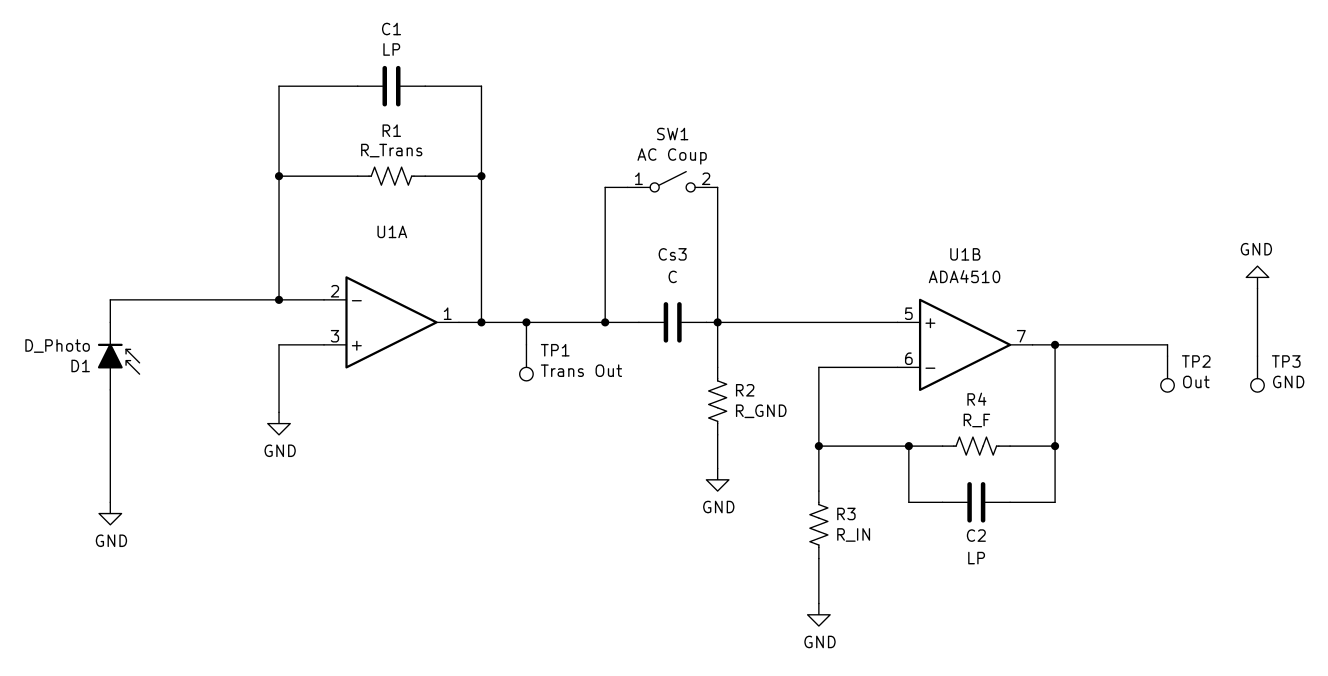
\includegraphics[width=1.0\linewidth]{diagrams/TIA_Schematic}
		\caption{Schematic of transimpedance amplifier board.}
		\label{fig:tiaschematic}
	\end{figure}
	
	\begin{figure}[H]
		\centering
		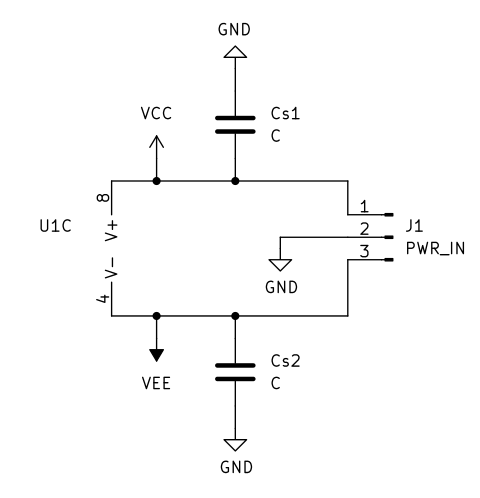
\includegraphics[width=0.35\linewidth]{diagrams/TIA_Power}
		\caption{Power Connections and decoupling capacitors for the amplifier board. The \texttt{Cs1} and \texttt{Cs2} are surface mount capacitors. \texttt{U1C} corresponds to the $\mathrm{V_{CC}}$ and $\mathrm{V_{EE}}$ connections of the op-amp \texttt{U1}.}
		\label{fig:tiapower}
	\end{figure}
	
	
	\subsection*{Resistor and Capacitor Selection for Transimpedance amplifier}
	There are three main parameters to choose in this design:
	\begin{itemize}
		\item Transimpedance gain, secondary gain
		\item Upper Cutoff frequency
		\item AC Coupling Cutoff frequency (optional)
	\end{itemize}
	The selection of these parameters is performed as follows.
	\subsubsection*{Transimpedance Gain}
	The value of \verb|R_Trans| gives the transimpedance value. For a photocurrent $I_p$ generated by the action of light on the photodiode, the output of the transimpedance amplifier will be
	\begin{equation*}
		V_\mathrm{Trans} = I_p \cdot R_\mathrm{Trans}
	\end{equation*}
	
	There is a second gain stage that can be configured for different gain values. The gain of this second stage is given in terms of \verb|R_F| and \verb|R_IN| as
	\begin{equation*}
		G_2 = 1 + \frac{R_\mathrm{F}}{R_\mathrm{IN}}
	\end{equation*}
	
	This second stage can be optionally configured as a unity gain buffer by omitting \verb|R_IN| and shorting \verb|R_F|. In this case, \verb|C2| can also be omitted.
	
	\textbf{Note}: When AC coupling is used, a gain of \textgreater 2$\times$ is needed to avoid premature saturation of the first stage when large signals are encountered.
	
	\subsubsection*{Upper Cutoff Frequency}
	The upper frequency cutoff is formed by three distinct single-pole filters, formed by the $RC$ time constants of:
	\begin{itemize}
		\item The first stage cutoff frequency, formed by the time constant \verb|R_Trans|$\times$\verb|C1|
		\item The second statge cutoff frequency, formed by the time constant \verb|R_F|$\times$\verb|C2|
		\item The photodiode internal capacitance, $C_p$, and the transimpedance: $C_p \times$ \verb|R_Trans|
	\end{itemize}
	Each of these three $RC$ time constants form a 1$^\mathrm{st}$ order filter with cutoff frequency
	\begin{equation*}
		f = \frac{1}{2\pi R C}
	\end{equation*}
	
	\subsubsection*{AC Coupling Frequency}
	The AC coupling feature of this design is optional an can be bypassed entirely by installing a jumper across \verb|Cs3|. This is also the job of the optional \verb|AC Coup| switch.
	
	When implemented, the AC coupling feature gives a high-pass cutoff frequency of $f = 1/(2\pi\times$\verb|R_GND|$\times$\verb|Cs3|$)$
	
	\subsubsection*{A Working Design}
	The following design is provided in Table \ref{tbl:TIA_design} as a working starting point. The transimpedance gain can be adjusted for different photodiodes. Sometimes it is possible to eliminate \verb|C1| if the op-amp stability permits. The internal capacitance of the photodiode is not shown here.
	
	\begin{table}[H]
		\begin{center}
			\caption{A working design for a 220k{\textohm} Transimpedance, 2$\times$ gain photodetector. The switchable AC coupling frequency is set to 3.3Hz, and the upper cutoff frequency is roughly 80KHz, but the response remains measurable to at least 150kHz. Tested with a Marktech Optoelectronics  \href{https://www.mouser.com/en/ProductDetail/Marktech-Optoelectronics/MTPD1346D-100?qs=DPoM0jnrROX\%252BgtLihG6RCQ\%3D\%3D}{MTPD1346D-100} InGaAs photodiode, and a \href{https://www.mouser.com/en/ProductDetail/Texas-Instruments/TL072CDR?qs=rshUhwi3fbas9IM4CCaZdw\%3D\%3D}{TI-072} op-amp.} \label{tbl:TIA_design}
			\begin{tabular}{|c|c|c|c|c|c|c|}
			\hline
			\verb|R_Trans| & \verb|C1|  & \verb|Cs3| & \verb|R_GND| & \verb|R_IN| & \verb|R_F| & \verb|C2| \\
			\hline
			220k\textohm & 10pF & 4.7{\textmu}F & 10k\textohm & 1k\textohm & 1k\textohm & 1.5nF \\
			\hline
		\end{tabular}
		\end{center}
	\end{table}
	
	\begin{table}[H]
		\begin{center}
			\caption{Links to Passive Component Sources} \label{tbl:TIA_parts}
			\begin{tabular}{|c|c|c|}
				\hline
				\verb|Cs3| & 4.7{\textmu}F Surface Mount Capacitor & \href{https://www.mouser.com/en/ProductDetail/Samsung-Electro-Mechanics/CL21A475KAQNNNF?qs=xZ\%2FP\%252Ba9zWqZ12ZgK1dMWug\%3D\%3D}{Mouser Link} \\
				\hline
				\verb|R_IN|, \verb|R_F| & 1k{\textohm} Resistor, 1\%, 100ppm & \href{https://www.mouser.com/en/ProductDetail/SEI-Stackpole/RNF14FTD1K00?qs=FESYatJ8odJnVtDgFQ4V9g\%3D\%3D}{Mouser Link} \\
				\hline
				\verb|R_GND| & 10k{\textohm} Resistor, 1\%, 50ppm & \href{https://www.mouser.com/en/ProductDetail/TE-Connectivity-Holsworthy/LR1F10K?qs=ip69W3eHERWDLLWs2Qv0Lg\%3D\%3D}{Mouser Link} \\
				\hline
			\end{tabular}
		\end{center}
	\end{table}
	
	\begin{table}[H]
		\begin{center}
			\caption{Operational amplifier IC selection guide for \texttt{U1}.} \label{tbl:TIA_opamp}
			\begin{tabular}{|c|c|c|}
				\hline
				TI-072 & The "Jelly Bean". Cheap, decent noise. & \href{https://www.mouser.com/en/ProductDetail/Texas-Instruments/TL072CDR?qs=rshUhwi3fbas9IM4CCaZdw\%3D\%3D}{Mouser Link} \\
				\hline
				OPA1678 & Lower Noise, Audiophile Grade. Rail-to-Rail Output  & \href{https://www.mouser.com/en/ProductDetail/Texas-Instruments/OPA1678IDR?qs=Mv7BduZupUj21oI9QX1tVA\%3D\%3D}{Mouser Link} \\
				\hline
			\end{tabular}
		\end{center}
	\end{table}

	\subsection*{The Amplifier Board}
	Solder the surface mounts first, using solder paste. After the four surface mount components are soldered, the passives can be hand-soldered with an iron.
	
	% Subfigures 
	\begin{figure} [h]
		\centering
		\begin{subfigure}{.5\textwidth}
			\centering
			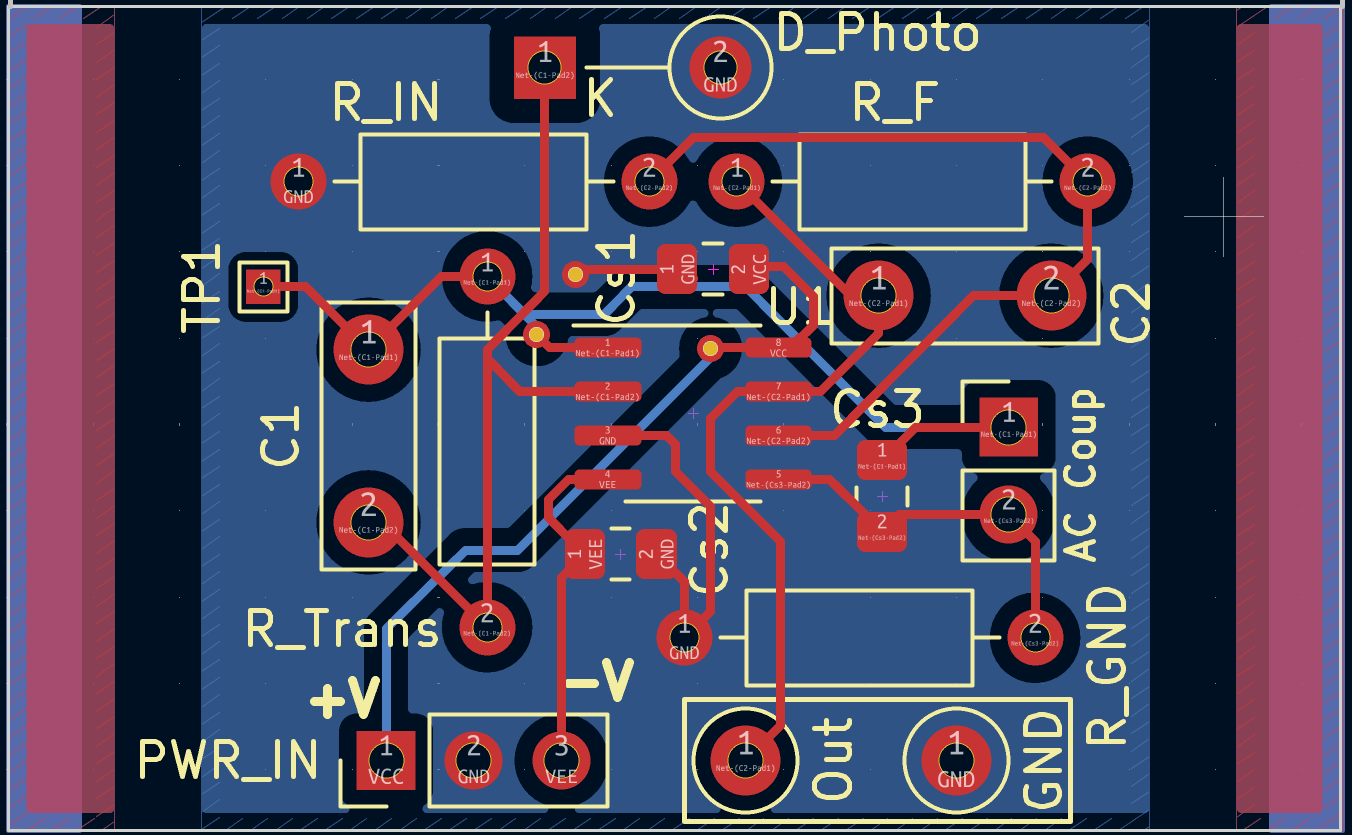
\includegraphics[width=0.85\linewidth]{diagrams/TIA_PCB_front}
			\caption{Front}
			\label{fig:sub1}
		\end{subfigure}%
		\begin{subfigure}{.5\textwidth}
			\centering
			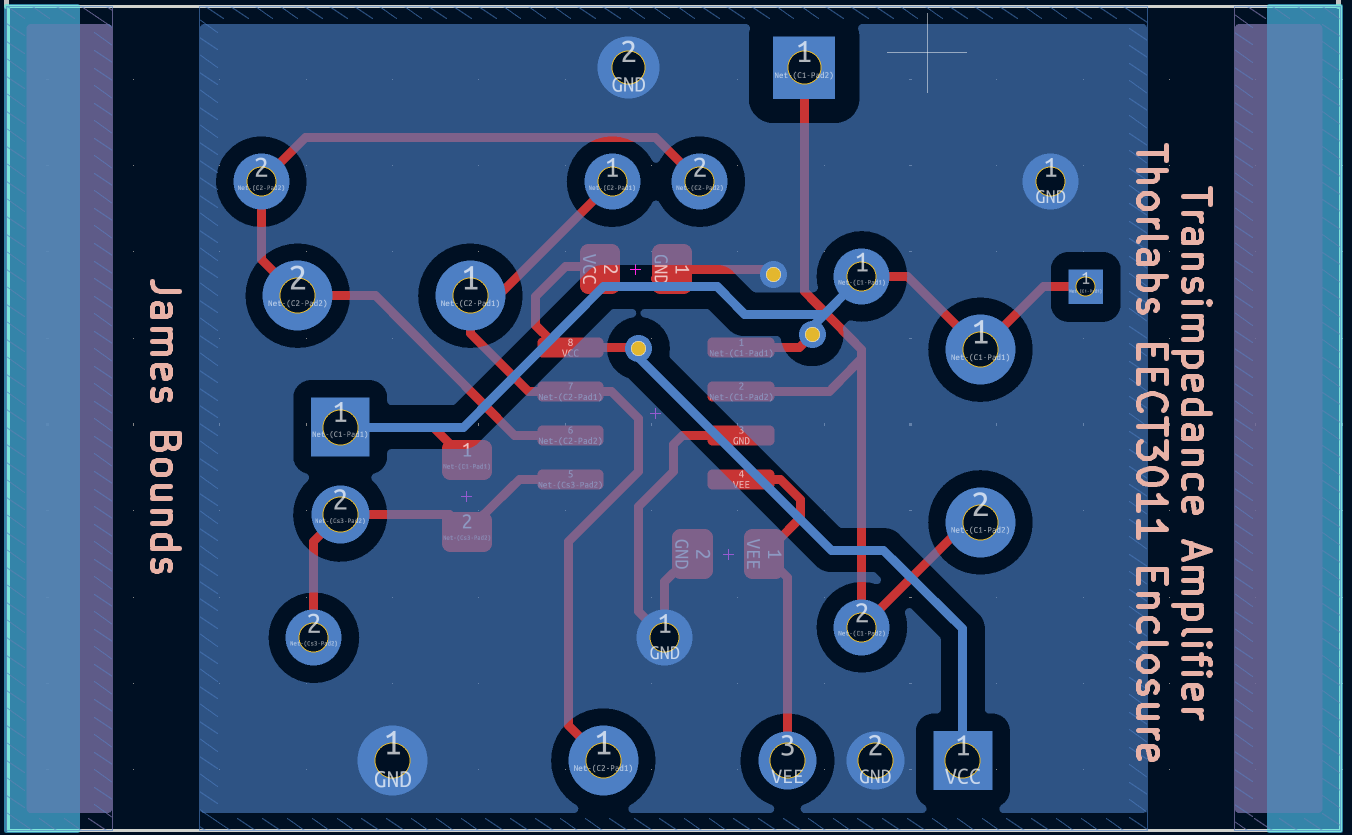
\includegraphics[width=0.85\linewidth]{diagrams/TIA_PCB_back}
			\caption{Back}
			\label{fig:sub2}
		\end{subfigure}
		\caption{Transimpedance amplifier PCB board.}
		\label{fig:test}
	\end{figure}
	
	\begin{figure}[H]
		\centering
		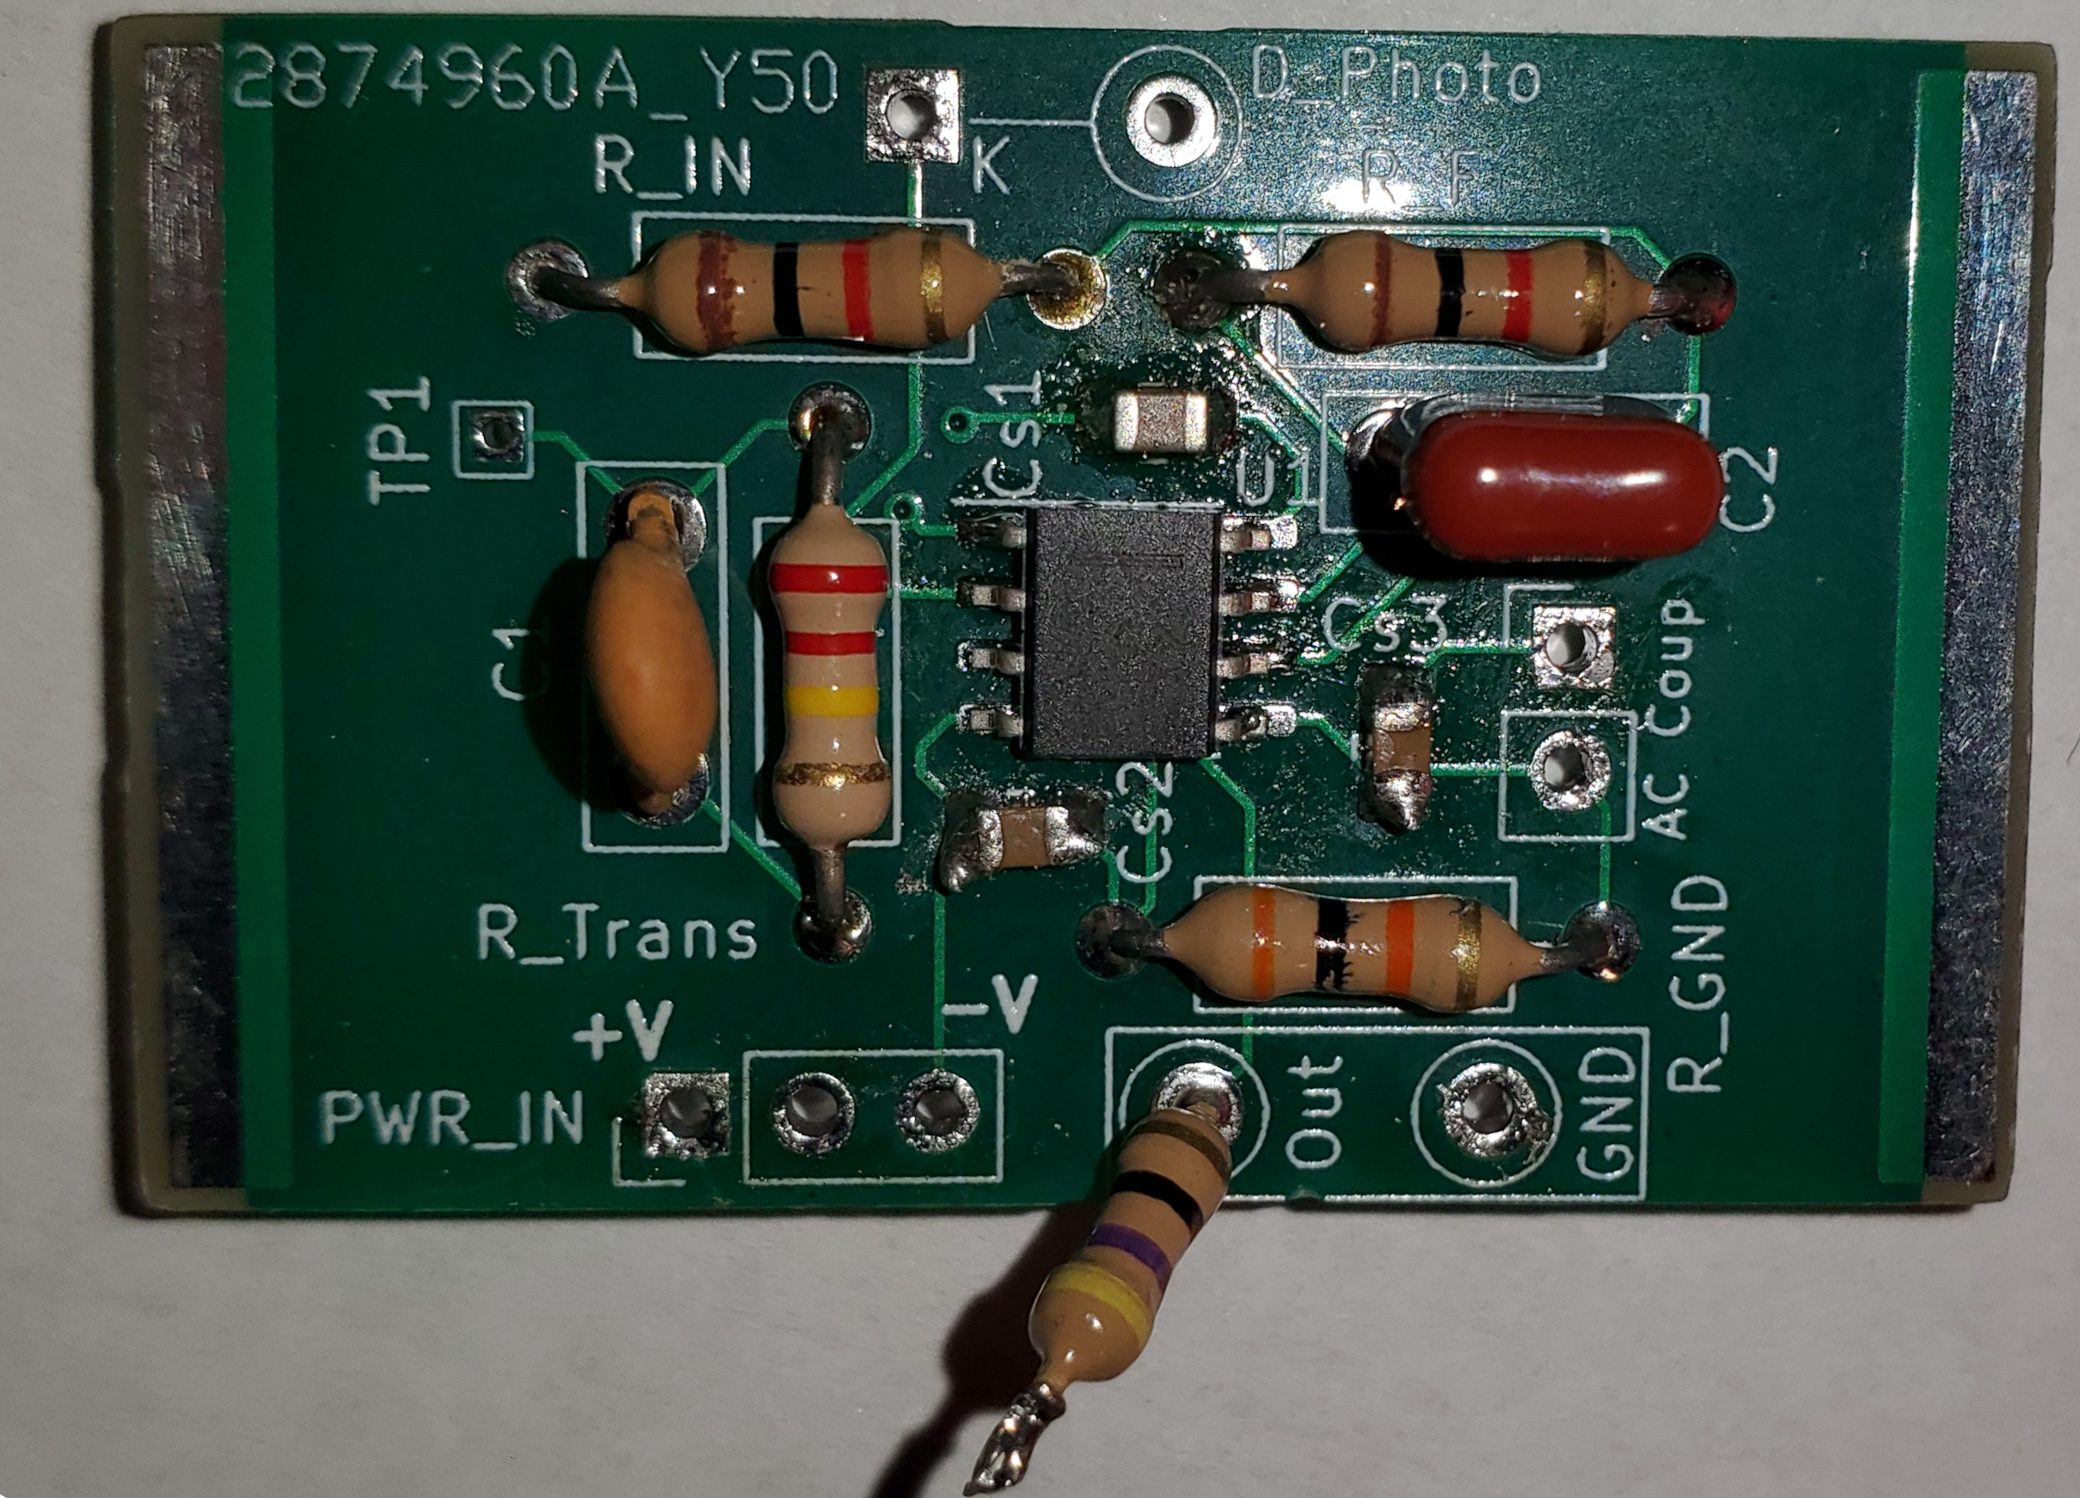
\includegraphics[width=0.5\linewidth]{diagrams/TIA_Pic}
		\caption{Soldered transimpedance amplifier board. An external 47{\textohm} resistor is shown connected in series with the output for short-circuit protection and impedance matching with a 50{\textohm} transmission line.}
		\label{fig:tiapic}
	\end{figure}
	
	\subsubsection*{Testing Notes}
	The amplifier board can be tested independently from the power supply circuit. This can be done by using an external $\pm$12V bipolar power supply.
	
	\section*{Power Supply Board}
	
	\begin{figure}[H]
		\centering
		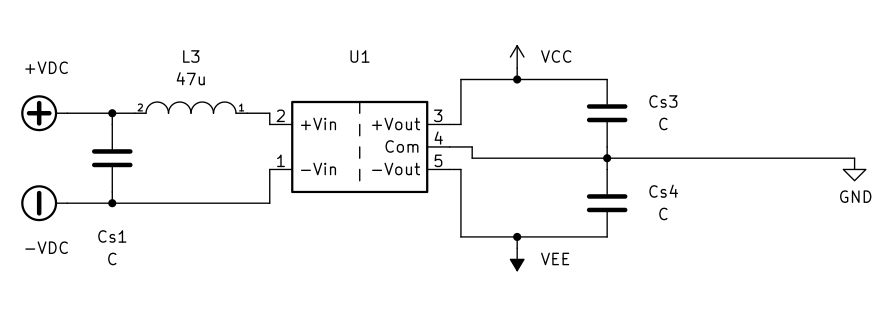
\includegraphics[width=0.7\linewidth]{diagrams/PS_Sch_conv}
		\caption{DC-DC converter section with filtering capacitors and inductor. For \texttt{U1}, a \href{https://www.mouser.com/en/ProductDetail/TRACO-Power/TRN-1-0523?qs=YCa\%2FAAYMW01OmFGNVe456Q\%3D\%3D}{TRACO Power TRN 1-0523} DC/DC converter is used. On the left are the 9V battery connections. The \texttt{VCC} and \texttt{VEE} are the dual outputs of the DC/DC converter.}
		\label{fig:psschconv}
	\end{figure}
	
	\begin{figure}[H]
		\centering
		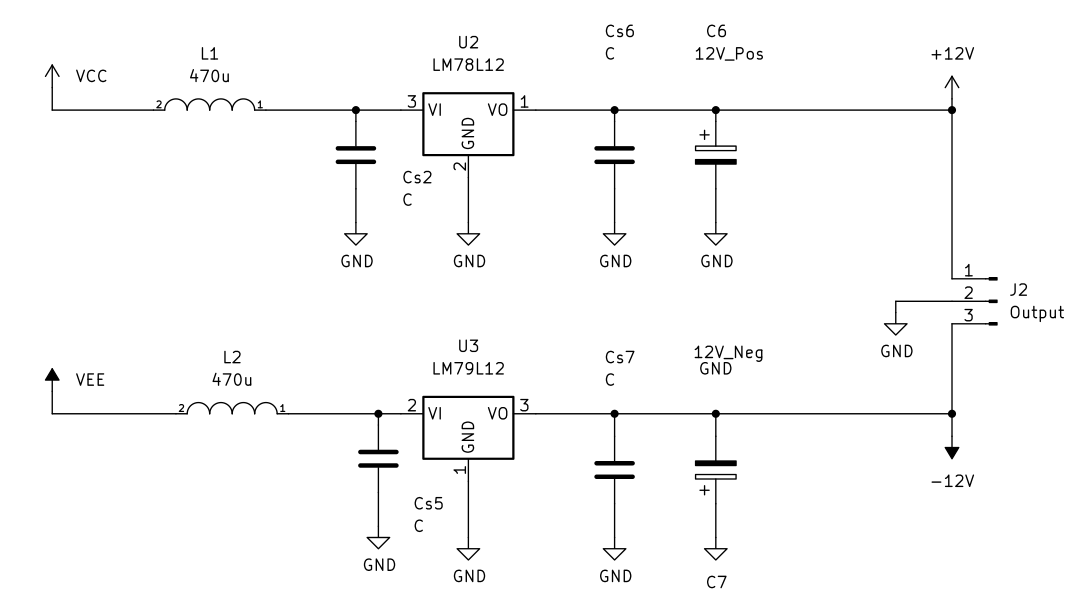
\includegraphics[width=0.85\linewidth]{diagrams/PS_Sch_reg}
		\caption{Regulator section schematic.}
		\label{fig:psschreg}
	\end{figure}
	
	\begin{figure}[H]
		\centering
		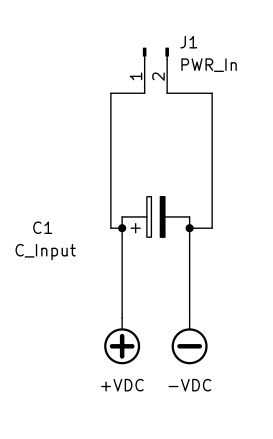
\includegraphics[width=0.2\linewidth]{diagrams/PS_Sch_conn}
		\caption{Battery input connector and battery input capacitor.}
		\label{fig:psschconn}
	\end{figure}
	
	
	\begin{table}[H]
		\begin{center}
			\caption{Links to component sources for power supply board}
			\begin{tabular}{|c|c|c|}
				\hline
				\verb|Cs*| & 4.7{\textmu}F Surface Mount Capacitor & \href{https://www.mouser.com/en/ProductDetail/Samsung-Electro-Mechanics/CL21A475KAQNNNF?qs=xZ\%2FP\%252Ba9zWqZ12ZgK1dMWug\%3D\%3D}{Mouser Link} \\
				\hline
				\verb|U1| & DC/DC Converter & \href{https://www.mouser.com/en/ProductDetail/TRACO-Power/TRN-1-0523?qs=YCa\%2FAAYMW01OmFGNVe456Q\%3D\%3D}{Mouser Link} \\
				\hline
				\verb|U2| & Fixed +12V Positive Voltage Regulator & \href{https://www.mouser.com/en/ProductDetail/Texas-Instruments/UA78L12ACLPR?qs=0O\%2FZFlpUpJUotYwhtoESdQ\%3D\%3D}{Mouser Link} \\
				\hline
				\verb|U3| & Fixed -12V Negative Voltage Regulator & \href{https://www.mouser.com/en/ProductDetail/Texas-Instruments/LM79L12ACZ-LFT4?qs=QbsRYf82W3GleqCHpRJpHQ\%3D\%3D}{Mouser Link} \\
				\hline
			\end{tabular}
		\end{center}
	\end{table}
	
	% Subfigures 
	\begin{figure} [h]
		\centering
		\begin{subfigure}{.5\textwidth}
			\centering
			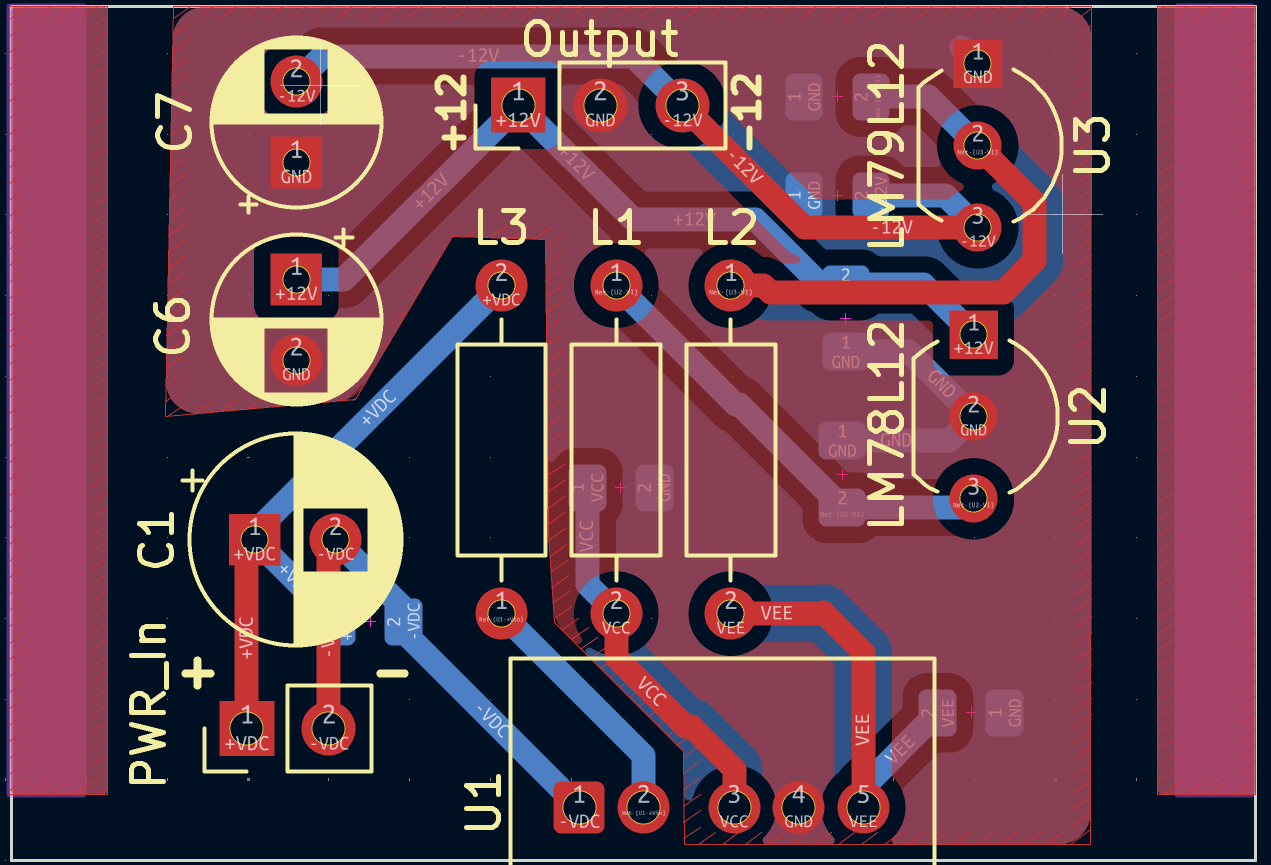
\includegraphics[width=0.85\linewidth]{diagrams/PS_PCB_front}
			\caption{Front}
		\end{subfigure}%
		\begin{subfigure}{.5\textwidth}
			\centering
			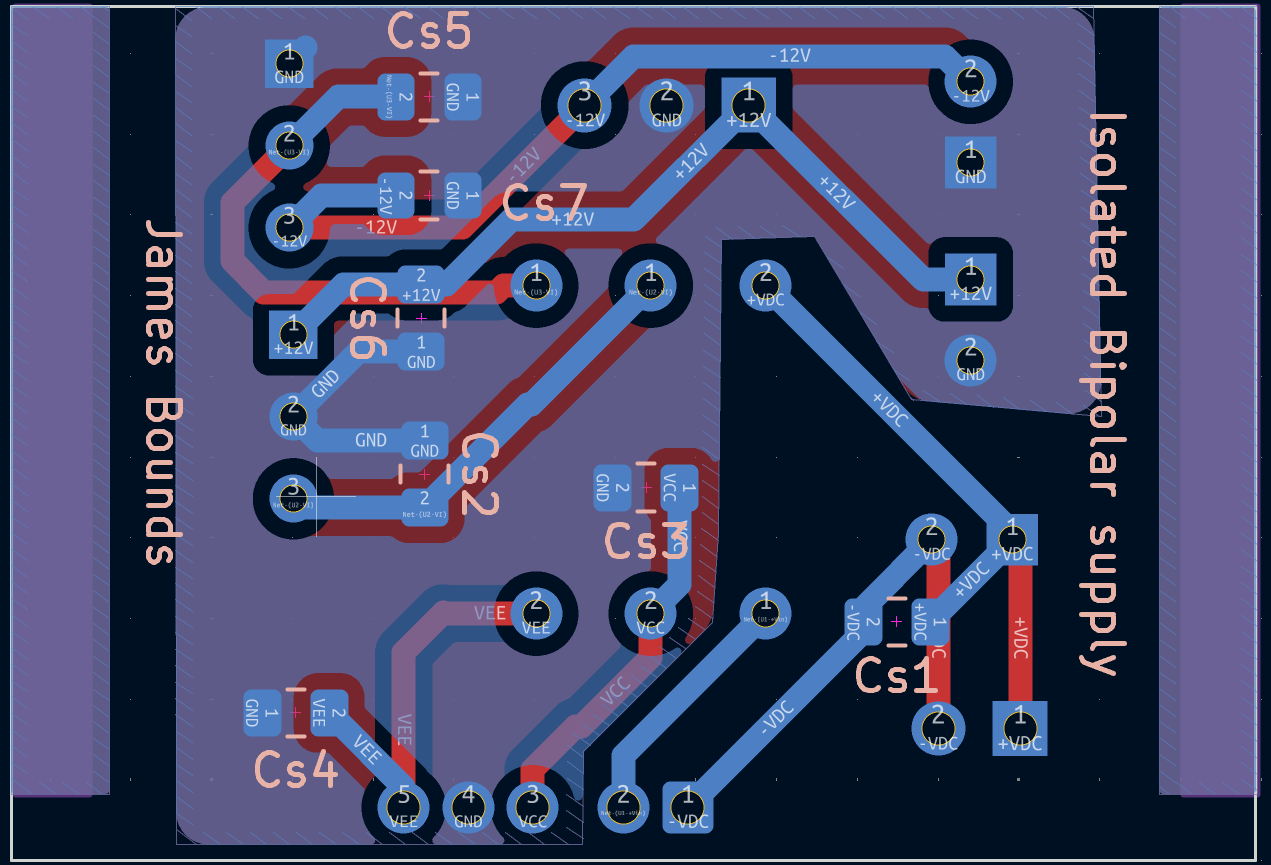
\includegraphics[width=0.85\linewidth]{diagrams/PS_PCB_back}
			\caption{Back}
		\end{subfigure}
		\caption{Power supply circuit PCB board.}
	\end{figure}
	
	\begin{figure}[H]
		\centering
		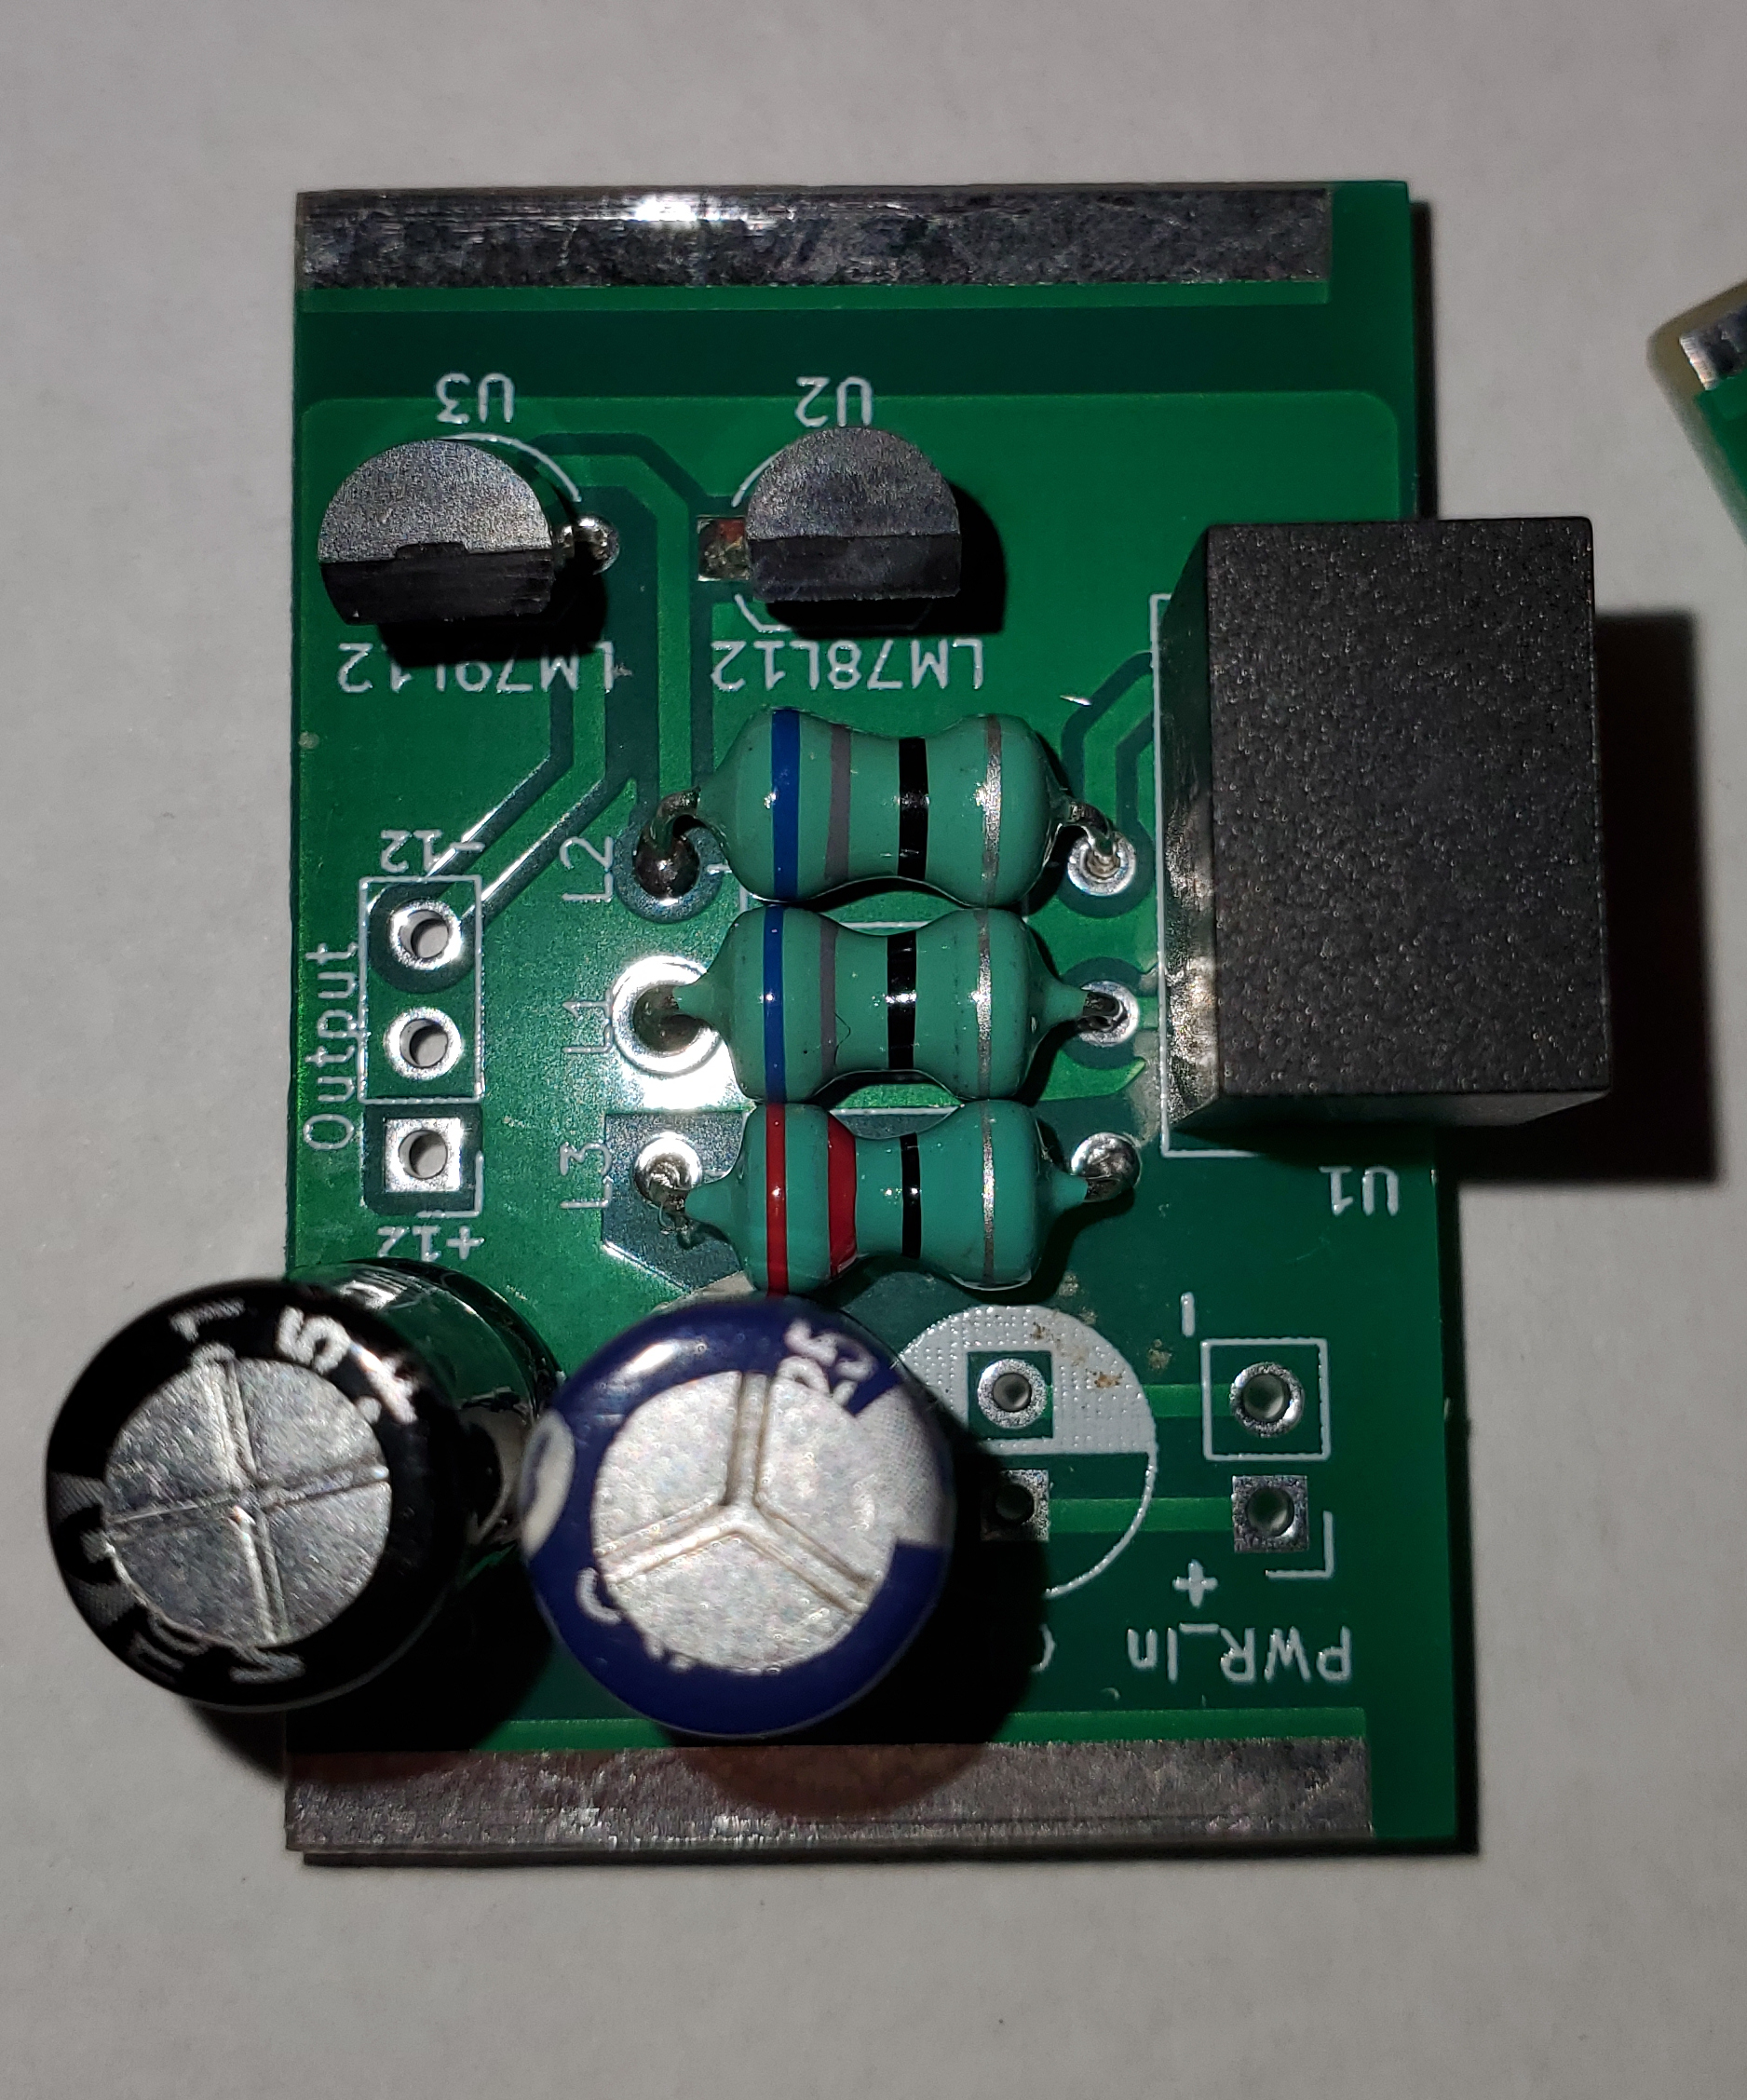
\includegraphics[width=0.4\linewidth]{diagrams/PS_Pic}
		\caption{Completed power supply board. The input capacitor is omitted here to increase viewing ability.}
		\label{fig:pspic}
	\end{figure}
	
	\section*{Photodetector Assembly}

\end{document}